%%========================================================================
%% LaTeX sjabloon voor stage/projectrapport of bachelorproef
%%  HoGent Bedrijf en Organisatie
%%========================================================================

%%========================================================================
%% Preamble
%%========================================================================

\documentclass[pdftex,a4paper,12pt,twoside]{report}

% XXX: Let op: dit sjabloon is gemaakt om dubbelzijdig af te drukken
% Voor enkelzijdig, verwijder ``twoside'' hierboven.

%%---------- Extra functionaliteit ---------------------------------------

\usepackage[utf8]{inputenc}  % Accenten gebruiken in tekst (vb. é ipv \'e)
\usepackage{amsfonts}        % AMS math packages: extra wiskundige
\usepackage{amsmath}         %   symbolen (o.a. getallen-
\usepackage{amssymb}         %   verzamelingen N, R, Z, Q, etc.)
\usepackage[dutch]{babel}    % Taalinstellingen: woordsplitsingen,
                             %  commando's voor speciale karakters
                             %  ("dutch" voor NL)
\usepackage{eurosym}         % Euro-symbool €
\usepackage{geometry}
\usepackage{graphicx}        % Invoegen van tekeningen
\usepackage{wrapfig}         % Positioneren van tekeningen
\usepackage[pdftex,bookmarks=true]{hyperref}
                             % PDF krijgt klikbare links & verwijzingen,
                             %  inhoudstafel
\usepackage{listings}        % Broncode mooi opmaken
\usepackage{multirow}        % Tekst over verschillende cellen in tabellen
\usepackage{rotating}        % Tabellen en figuren roteren
\usepackage{natbib}          % Betere bibliografiestijlen
\usepackage{fancyhdr}        % Pagina-opmaak met hoofd- en voettekst

\usepackage[T1]{fontenc}     % Ivm lettertypes
\usepackage{lmodern}
\usepackage{textcomp}
\usepackage{listings}


%%---------- Layout ------------------------------------------------------

% hoofdingen, enz.
\pagestyle{fancy}
% enkel hoofdstuktitel in hoofding, geen sectietitel (vermijd overlap)
\renewcommand{\sectionmark}[1]{}

% lijn, wordt gebruikt in titelpagina
\newcommand{\HRule}{\rule{\linewidth}{0.5mm}}

% Leeg blad
\newcommand{\emptypage}{
\newpage
\thispagestyle{empty}
\mbox{}
\newpage
}

% Gebruik een schreefloos lettertype ipv het "oubollig" uitziende
% Computer Modern
\renewcommand{\familydefault}{\sfdefault}

%%---------- Documenteigenschappen ---------------------------------------
%% Vul dit aan met je eigen info:

% Je eigen naam
\newcommand{\student}{Michiel De Wilde}

% De naam van je lector, begeleider, promotor
\newcommand{\promotor}{Bert Van Vreckem}

% De naam van je co-promotor
\newcommand{\copromotor}{Micha Hernández van Leuffen}

% Indien je bachelorproef in opdracht van een bedrijf of organisatie
% geschreven is, geef je hier de naam.
\newcommand{\instelling}{Hogeschool Gent}

% De titel van het rapport/bachelorproef
\newcommand{\titel}{Vergelijking van unikernel-implementaties}

% Datum van indienen
\newcommand{\datum}{29 mei 2015}

% Faculteit
\newcommand{\faculteit}{Faculteit Bedrijf en Organisatie}

% Soort rapport
\newcommand{\rapporttype}{Scriptie voorgedragen tot het bekomen van de graad van\\Bachelor in de toegepaste informatica}

% Academiejaar
\newcommand{\academiejaar}{2015-2016}

% Examenperiode
%  - 1e semester = 1e examenperiode
%  - 2e semester = 2e examenperiode
%  - tweede zit = 3e examenperiode
\newcommand{\examenperiode}{2e examenperiode}

%%========================================================================
%% Inhoud document
%%========================================================================

\begin{document}

%%---------- Front matter ------------------------------------------------
%% Het voorblad - Hier moet je in principe niets wijzigen.

\begin{titlepage}
  \newgeometry{top=2cm,bottom=1.5cm,left=1.5cm,right=1.5cm}
  \begin{center}

    \begingroup
    \rmfamily
    
\includegraphics[width=2.5cm]{img/HG-beeldmerk-woordmerk}\\[.5cm]
    \faculteit\\[3cm]
    \titel
    \vfill
    \student\\[3.5cm]
    \rapporttype\\[2cm]
    Promotor:\\
    \promotor\\
    Co-promotor:\\
    \copromotor\\[2.5cm]
    Instelling: \instelling\\[.5cm]
    Academiejaar: \academiejaar\\[.5cm]
    \examenperiode
    \endgroup

  \end{center}
  \restoregeometry
\end{titlepage}

% Schutblad

\emptypage


\begin{titlepage}
  \newgeometry{top=5.35cm,bottom=1.5cm,left=1.5cm,right=1.5cm}
  \begin{center}

    \begingroup
    \rmfamily
    \faculteit\\[3cm]
    \titel
    \vfill
    \student\\[3.5cm]
    \rapporttype\\[2cm]
    Promotor:\\
    \promotor\\
    Co-promotor:\\
    \copromotor\\[2.5cm]
    Instelling: \instelling\\[.5cm]
    Academiejaar: \academiejaar\\[.5cm]
    \examenperiode
    \endgroup

  \end{center}
  \restoregeometry
\end{titlepage}


\begin{abstract}

Het efficiënt gebruiken van de middelen die ter beschikking worden gesteld is vanzelfsprekend. Doorheen de tijd zijn er innovaties gekomen om dit steeds naar een hoger niveau te tillen bij software ontwikkeling en systeembeheer. Eerst was er sprake van virtuele machines en dan later kwamen software containers ter sprake. In de sector van informatica is stilstaan gelijk aan achteruit gaan. Het gemak en gebruikvriendelijk is een andere focus van deze innovaties. 

Unikernels is een opkomende manier voor het maken en gebruiken van programma's in een productieomgeving. Diverse onderwerpen zoals besturingssystemen worden nader bekeken of er geen verbeteringen kunnen gemaakt worden. Unikernels vraag om een andere kijk op programma's in de productieomgeving en hoe er gewerkt wordt met de architectuur en infrastructuur. Deze bachelorproef focust op de rol van de systeembeheerder binnen een architectuur van unikernels. Er wordt nader gekeken naar de competenties van systeembeheerder binnen dit soort architectuur. Ook de vergelijking tussen containers en unikernels wordt gemaakt. Verder bekijken we huidige implementaties van unikernels om een beter beeld te krijgen op het ecosysteem rond unikernels.

\end{abstract}

\chapter*{Voorwoord}
\label{ch:voorwoord}

Deze bachelorproef is tot stand gekomen uit eigen interesse. Computers hebben mij sinds mijn jeugd al gefascineerd. Het heeft een tijd geduurd vooraleer ik begon met programmeren. Ik begon met de simpele applicatie maar al snel werd het meer complex.  Het beheren van servers en infrastructuur was een uitdaging die ik zeker aanging. De traditionele server maakten plaats voor containers en daar begon voor mij zoektocht naar het beter en efficïenter gebruik maken van de middelen in een omgeving. Ook gemak was een factor die meespeelde. Een paar maanden voor mijn bachelorproef kwam ik het concept van unikernels tegen. Dit leek mij een goed onderwerp voor mijn bachelorproef en was ook al als onderwerp beschikbaar gesteld. Het was een mooie uitdaging om meer te leren over concepten rond systeembeheer en software ontwikkeling. Ik hoop dat deze bachelorproef beantwoord aan de verwachtingen en dat er veel uit kan geleerd worden.

Ik wens dhr. Van Vreckem te bedanken voor de begeleiding voor de bachelorproef.

Verder bedank ik de werknemers van mijn stageplaats, Wercker BV. In het bijzonder Toon Verbeek, Micha Hernández van Leuffen en Benno van den Berg. De bachelorproef zou er niet gekomen zonder hun hulp.

\tableofcontents

\chapter{Inleiding}
\label{ch:inleiding}

Bij het opleveren van software gaat eerst de software eerst lokaal ontwikkelt worden. Wanner de software opgeleverd wordt dan zal het geplaatst worden in een productieomgeving. Deze omgeving kan van de klant of het bedrijf dat de software ontwikkelt heeft zijn. Het geschreven programma van de lokale ontwikkelomgeving naar de productieomgeving brengen is de rol van de systeembeheerder. De productieomgeving bestaat uit servers die zich lokaal in het bedrijf bevinden of bij een cloud provider.

De middelen van de productieomgeving moet zo goed mogelijk gebruikt worden. In deze bachelorproef zullen we bekijken welke technologieën er kunnen gebruikt worden om dit te realiseren.

Deze bachelorproef behandelt het onderwerp unikernels (\cite{mao_performance_2012}) en wat voor gevolgen unikernels kunnen hebben op de taak van de systeembeheerder. De omgeving waarin wordt gewerkt kan verschillen van situatie tot situatie. Daarom is het aantonen van de situaties waarin unikernels kunnen gebruikt worden van uiterst belang.

De bachelorproef zal proberen de veranderingen te beschrijven. Dit is alleen mogelijk vanuit een blik op de huidige situatie. Sommige innovaties kunnen een groot gevolg hebben terwijl die nu nog niet aanwezig zijn.

In hoofdstuk 2 wordt de methodologie van de bachelorproef aangehaald.

Virtualisatie vormt de basis voor veel van de technologieën die worden aangehaald. Virtualisatie zal belicht worden in hoofdstuk 3.

Op 21 maart 2013 werd op Pycon de eerste demo van Docker gegeven (\cite{hykes_future_2013}). Het gegeven van containers bestond al langer, maar is pas echt doorgebroken onder Docker. In hoofdstuk 4 worden containers en Docker nader bekeken.

Hoofdstuk vijf dat unikernels behandelt, zal zich focussen op de werking van het concept, de voordelen en de implementaties van unikernels.

Verder zullen we kijken naar de veranderingen op het vlak van architectuur van programma's en infrastructuur. Dit beperkt zich niet tot unikernels want de meeste toepassingen kunnen ook mogelijk zijn met containers. Hoofdstuk zes is bedoeld om concepten aan te halen die veel op de voorgrond zullen treden wanneer containers en unikernels alomtegenwoordig zijn.

Hoofdstuk zeven zal de experimenten behandelen.

Uiteindelijk zullen we een conclusie trekken over de plaats van unikernels tegenover bestaande alternatieven en de gevolgen voor systeembeheerders wanneer unikernels meer maturiteit verkrijgen.

\section{Probleemstelling en Onderzoeksvragen}
\label{sec:onderzoeksvragen}

Het doel van deze bachelorproef is om de veranderingen voor de systeembeheerder aan te tonen wanneer unikernels meer gebruikt zullen worden.
Dit zal gebeuren door de volgende onderzoeksvragen te beantwoorden:

\begin{itemize}  
\item Zullen de competenties van de systeembeheerder veranderen?
\item Wordt het opzetten van applicaties eenvoudiger of niet?
\item We kunnen wel spreken over de opvolger van containers maar is deze al werkbaar in de toekomst?
\item Wat is de impact op beveiliging, meer bepaald aspecten als beschikbaarheid, autorisatie, integriteit en vertrouwelijkheid van gegevens?
\end{itemize}

\chapter{Methodologie}
\label{ch:methodologie}

Het begrip unikernel vraagt om een uitgebreide theoretische kennis van besturingssystemen en virtualisatietechnologieën.

Om veel van deze concepten goed te begrijpen werd er eerst een literatuurstudie uitgevoerd.
Een belangrijk beginpunt was de volgende website (\cite{unikernel_systems_unikernels_2016}). De voorgenoemde website heeft een lijst van papers over unikernels en verwijzingen naar implementaties van unikernels.
Veel over virtuele machines was te vinden in thesissen van de vorige jaren van de opleiding toegepaste informatie. De kennis over containers werd voornamelijk opgedaan tijdens mijn stage bij Werker. Een paar boeken over containers, met centraal onderwerp Docker, gaven meer inzicht in containers en hun use cases.

De literatuurstudie vormde de basis voor de eerste hoofdstukken over virtuele machines, containers en unikernels. De bachelorproef focust niet alleen op de mogelijkheden die unikernels hebben, ook de eventuele gevolgen voor systeembeheerders moeten bekeken worden.

Het hoofdstuk na unikernels maakt een vergelijking tussen de implementaties van unikernels op het vlak van gemak, inzetbaarheid en mogelijkheden. Hiervoor werd er veel opzoekwerk gedaan om de gegevens van de implementaties te vinde.

Microservices en Immutable Infrastructure zijn twee gegevens die bekend aan het worden zijn binnen de wereld van systeembeheer en software ontwikkeling. Dit leidde tot een hoofdstuk die hun verband aantoonde met unikernels en containers. De revolutie voor software ontwikkeling en systeembeheerders door deze soort technologieën te gebruiken geeft een duidelijk beeld op de gevolgen voor systeembeheerders.

\chapter{Virtualisatie}
\label{ch:virtualisatie}

In dit hoofdstuk zal bekeken worden waarom en hoe virtualisatie ontstaan is. Verder zal bekeken worden welke concepten meespelen binnen virtualisatie. Dit hoofdstuk dient als een inleiding om concepten zoals containers, unikernels en virtuele machines te kunnen begrijpen.

In de jaren 60 was de tijd dat je een computer kon gebruiken beperkt (\cite{conferences_modern_1968}).  Bij de eerste computers had men problemen om programma's uit te werken. Dit lag vooral aan de tijd dat je kon werken aan de computer. Er waren vele mensen die aan één computer aan het werken waren en dit zorgde voor een tijdsnood. Een voorbeeld van het ontwikkelen van een programma in die tijd was de volgende: "De broncode van het programma werd ingegeven en in een wachtrij geplaatst. Pas een bepaalde tijd later kon men de resultaten van het programma bekijken. Fouten in het geschreven programma zorgen voor een groot tijdsverlies." (\cite{conferences_modern_1968})

Eén van de grootste bijdrage tot de ontwikkelsnelheid van programma's is de lengte van de feedbackcyclus: hoe snel kan een programma getest worden wanneer er een verandering gebeurd. Als een paar minuten moet worden gewacht op het testen van een kleine verandering, dan is dit niet ideaal. Dit leidt tot een verlies van tijd en dus geld.

timesharing (\cite{pyke_jr._time-shared_1967}) werd uitgevonden om het verlies van voorgenoemde tijd te beperken. Bij timesharing kunnen gebruikers inloggen op een console en zo tegelijk van de computer gebruik maken. Dit was een technische uitdaging. Elke gebruiker en zijn programma's bevinden zich binnen een afzonderlijke context. De computer zou van de ene context naar de andere moeten kunnen veranderen. Timesharing zou de basis vormen voor het moderne besturingssysteem. Eén van de moeilijkheden van timesharing is de isolatie van twee verschillende processen. De twee processen moeten zich bevinden binnen een verschillende context. Deze contexten mogen niet met elkaar in contact komen of elkaar niet beïnvloeden.

Doorheen de tijd kregen de computers meer middelen. De meeste programma's konden niet langer de alle middelen van de computer benutten. Dit zorgde voor de creatie van virtuele middelen of virtual resources (\cite{vakilinia_modeling_2015}). Om deze virtuele middelen te voorzien moeten bepaalde delen van de computer gevirtualiseerd worden. Dit kan voorkomen als verschillende vormen zoals hardware virtualisatie en virtualisatie van het besturingssysteem.

\begin{wrapfigure}{r}{0.3\textwidth}
    \centering
    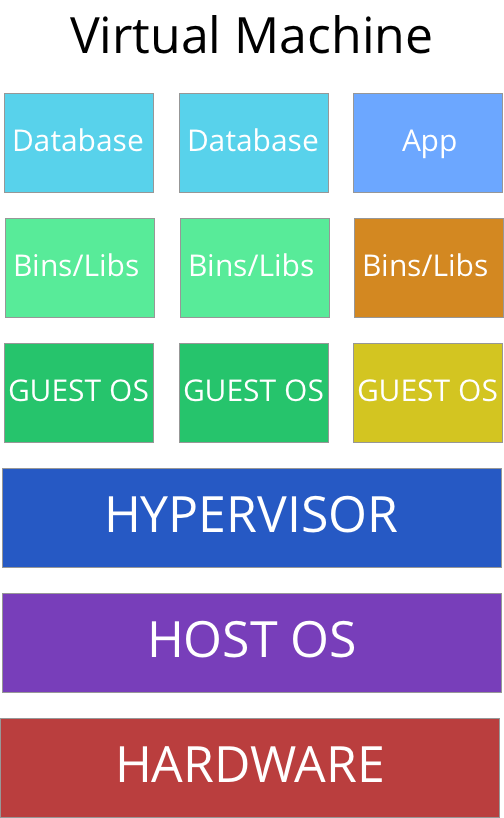
\includegraphics[width=3cm]{img/virtual-machine}
    \caption{structuur van een virtuele machine}
    \label{fig:virtualmachine}
\end{wrapfigure}

Het concept van virtualisatie deelt een aantal gelijkenissen met timesharing. De computer wordt opgedeeld in verschillende delen bij virtualisatie en bij timesharing gaan we de computer opdelen in contexten. De verschillende delen bij beide concepten moeten ook geïsoleerd zijn van elkaar.

Een aantal voordelen van virtualisatie zijn de volgende: financieel voordeel (men kan van één taak naar meerdere taken gaan op één computer), besparen van energie (\cite{beloglazov_energy_2010}) en veiligheid(\cite{mortleman_security_2009}).

Een virtuele machine (\cite{smith_architecture_2005}) bootst een computer na. Het laat toe om een besturingssysteem te gebruiken, wanneer de hardware van de fysieke computer dit niet toelaat. Een virtuele machine kan ook de middelen van de fysieke computer waar het zich op bevindt gebruiken. Dit zorgt ervoor dat de middelen van de fysieke computer kunnen gebruikt worden als virtuele middelen. De fysieke computer zal verder naar verwezen worden als de host machine. Guest is de naam dat we geven aan virtuele machines die zich bevinden op de host. In het volgende deel zullen we de laag tussen de host machine en virtuele machine bekijken: de hypervisor. Figuur \ref{fig:virtualmachine} toont de structuur van een virtuele machine. 

\section{Hypervisor}

Een hypervisor (\cite{popek_formal_1974}) is een voorbeeld van hardware virtualisatie. Het is een stuk software, firmware of hardware dat de laag vormt tussen de virtuele machine en de host machine. De host machine zorgt voor de middelen zoals CPU, RAM, ... Elke virtuele machine die zich bevindt op de host machine zal dan gebruik maken van een gedeelte van deze middelen. Doordat virtualisatie alomtegenwoordig geworden is in datacenters (\cite{soundararajan_impact_2010}) heeft het ervoor gezorgd dat er meer logica komt te liggen bij de hypervisor. De hypervisor neemt verder de rol op zich van het verdelen van de middelen en het beheren van de guests. Er zijn twee soorten hypervisors: type 1 en type 2. Type 1 is de bare-metal hypervisor en type 2 de hosted hypervisor. De volgende twee delen zullen deze twee types uitleggen.

\newpage

\subsection{Hosted Hypervisors}

\begin{wrapfigure}{r}{0.3\textwidth}
    \centering
    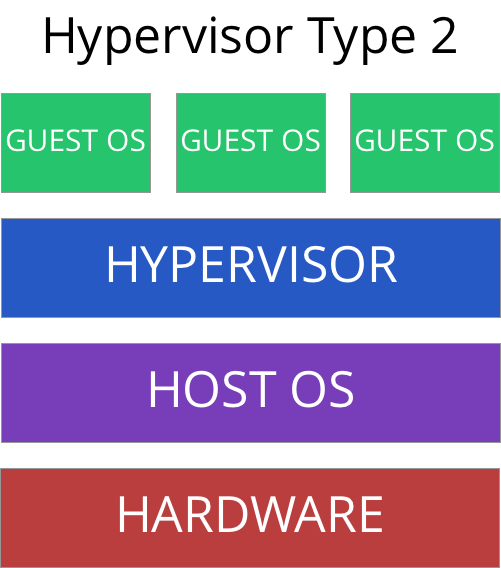
\includegraphics[width=3cm]{img/hypervisor-2}
    \caption{structuur van een hosted hypervisor}
    \label{fig:hypervisor-2}
\end{wrapfigure}

Als eerste zullen we de hosted hypervisor of type 2 hypervisor behandelen. Figuur \ref{fig:hypervisor-2} toont de structuur van een hosted hypervisor. De hosted hypervisor bevindt zich op het besturingssysteem van de host machine en heeft geen directe toegang tot de hardware. De type 2 hypervisor compleet afhankelijk van het besturingssysteem van de host om zijn taken uit te voeren. Als er problemen optreden in het besturingssysteem van de host zijn er gevolgen voor de hypervisor en guests.

Voorbeelden van hosted hypervisors zijn: Oracle Virtualbox (\cite{oracle_oracle_2016}) en VMware Workstation (\cite{vmware_vmware_2016-1}).

\subsection{Bare-metal Hypervisors}

\begin{wrapfigure}{l}{0.3\textwidth}
    \centering
    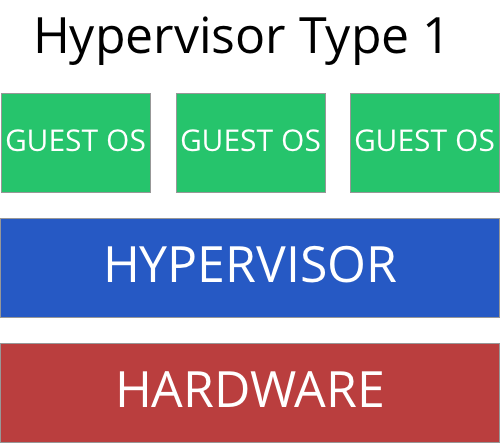
\includegraphics[width=3cm]{img/hypervisor-1}
    \caption{structuur van een bare-metal hypervisor}
    \label{fig:hypervisor-1}
\end{wrapfigure}

Type 1, bare-metal, embedded of native hypervisors bevinden zich rechtstreeks op de hardware. De voornaamste taak van de hypervisor is het beheren en delen van hardware middelen. Dit maakt de hardware hypervisor kleiner in omvang dan de hosted hypervisor. De hypervisor heeft niet het probleem van de hosted hypervisor dat er grote problemen kunnen liggen bij het besturingssysteem van de host. Dit is omdat de hypervisor niet berust op een besturingssysteem. Figuur \ref{fig:hypervisor-1} toont de structuur van een bare-metal hypervisor.

Er is een laag minder in de structuur dus dit betekent dat er minder instructies moeten worden uitgevoerd  bij een bepaalde handeling. Dit heeft een beter prestatie tot gevolg. Omdat er geen problemen kunnen zijn met het besturingssysteem van de host kunnen we aannemen dat deze soort hypervisor stabieler is. Wanneer het besturingssysteem van de host faalt bij een hosted hypervisor dan zullen de guests ook falen.

Een paar voorbeelden van bare-metal hypervisors zijn VMware ESXi (\cite{vmware_vmware_2016}) en Xen (\cite{xen_project_xen_2016}).

\section{Operating System-level Virtualization}

Naast hardware virtualisatie kan ook een besturingssysteem gevirtualiseerd worden. Bij deze toepassing van virtualisatie worden de mogelijkheden van de kernel gebruikt. De kernel van bepaalde besturingssystemen laat toe om meerdere geïsoleerde name spaces tegelijkertijd te laten werken. Dit zorgt ervoor dat de dat er maar één besturingssysteem moet zijn om verschillende programma's naast elkaar en geïsoleerd van elkaar te laten werken.

De name spaces maken gebruik van de middelen van de host. Elke name space heeft zijn eigen configuratie omdat de user spaces op zichzelf staan en geïsoleerd zijn van de andere user spaces. Dit geeft eveneens de beperking dat guests een besturingssysteem of kernel moeten hebben die overeenkomt met de host.

Tegenover hardware virtualisatie zal besturingssysteem virtualisatie minder gebruik maken van middelen omdat er maar één besturingssysteem is. Dit is omdat het besturingssysteem wordt gedeeld. Dit geeft voordelen bij de prestatie.

Voorbeelden van besturingssysteem virtualisatie zijn: chroot (\cite{linux_chroot2_????}), Solaris Containers (\cite{oracle_solaris_2016}) en Docker (\cite{docker_docker_2016}).

Besturingssysteem virtualisatie is vooral bekend geworden door Docker vanaf 2013 (\cite{hykes_future_2013}). In het volgende hoofdstuk wordt verder ingegaan op containers en Docker.

\chapter{Containers}
\label{ch:Containers}

\section{Containers}

\begin{wrapfigure}{l}{0.3\textwidth}
    \centering
    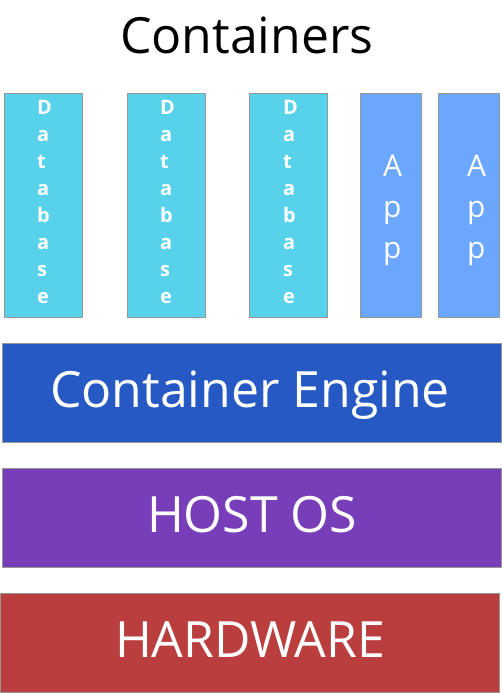
\includegraphics[width=3cm]{img/container}
    \caption{structuur van containers}
    \label{fig:containers}
\end{wrapfigure}

Containers bestaan al een tijd. In \cite{soltesz_container-based_2007} werd al gekeken naar de voordelen van containers tegenover hypervisors. Chroot (\cite{Linux}) is een concept dat veel deelt met containers. Chroot zal de root directory van het huidige proces en zijn children veranderen. Er wordt een virtuele kopie gemaakt van het systeem waarin het proces kan werken. Het proces is dus afgesloten van het systeem en dit zorgt voor meer veiligheid bij het uitvoeren van processen.

Linux Containers of LXC (\cite{containers_linux_????}) is een implementatie van besturingssysteem virtualisatie. LXC kan meerdere geïsoleerde Linux systemen laten werken op één host. Deze geïsoleerde Linux systemen worden containers genoemd. Deze containers worden ook getoond in figuur \ref{fig:containers} waarbij de apps en databases containers zijn. Het volgende deel van deze sectie zal de onderdelen van LXC uitleggen en de voordelen.

Zoals we al gezien hebben is de rol van de hypervisor het delen en beheren van de middelen. Om containers te gebruiken moeten iets anders de rol hiervan overnemen. Cgroups is een Linux kernel extension die deze rol overneemt. Door cgroups kunnen we middelen beheren voor processen tot en met containers. Het toont ook de mogelijkheden om checkpoints te creëren van processen.

Eerder werd ook al aangehaald dat de processen van elkaar gescheiden moeten worden. Dit wordt bereikt door name spaces. De functies die name spaces voorziet zijn uitgebreid. Elke name space heeft zijn eigen file system structure, netwerk interfaces en proces ID space. De containers delen de kernel met alle andere processen die op de kernel aan het werken zijn.

De containers zijn van elkaar afgesloten. Wanneer één container aangetast wordt dan heeft dit geen gevolg op de andere containers.

Toch zijn er een paar andere problemen zoals aangehaald in \cite{madhavapeddy_jitsu:_2015}. Processen die als root werken kunnen niet geïsoleerd worden van elkaar. Verder wordt er ook aangehaald dat strengere isolatie nodig is. (tabel 2, \cite{madhavapeddy_jitsu:_2015})

\section{Docker}

Docker (\cite{docker_docker_2016}) is een open source project om software containers te gebruiken voor programma's gemakkelijk op te stellen. Docker is eveneens het bedrijf dat al de delen samenbracht in een uitgebreid ecosysteem. Docker maakte de handelingen rond containers simpeler en intuïtief. Het werd gemakkelijk om containers te maken en te delen met anderen. Door veel van de componenten van het ecosysteem open te stellen voor het publiek konden ze rekenen op de steun van vele open source ontwikkelaars.

Er waren andere formaten dan Docker zoals rkt \cite{_rkt_????} die het mogelijk maakte voor containers te maken. Maar door hun ecosysteem en de hulp van de open source gemeenschap hebben is Docker de meest populair optie \cite{oreilly_media_docker_2015} geworden om met software containers te werken.

In 2015 werd het Open Container Initiative opgericht. Veel grote spelers op vlak van software containers zoals Docker, CoreOS, Microsoft en Google maken hier deel van uit. Samen willen ze een standaard voor software containers vastleggen. \cite{}.

De problemen die we bij software containers tegenkomen hebben voornamelijk betrekking tot beveiliging. Unikernels kan een veiliger alternatief zijn. In het volgende hoofdstuk bekijken we de werking en mogelijkheden met unikernels.

\chapter{Unikernels}
\label{ch:unikernels}

\section{Inleiding}

Dit hoofdstuk zal uitleggen uit welke delen een unikernel bestaat en een beter beeld geven op de voordelen van unikernels. De eigenschappen worden ook angehaald. In het volgende hoofdstuk wordt bekeken welke implementaties van unikernels er al bestaan en wat de verschillen ertussen zijn.

Virtuele machines (hoofdstuk \ref{ch:virtualisatie}) zijn er gekomen wanneer men de middelen van computers beter wou gebruiken. Toch werden de middelen niet optimaal benut door de besturingssystemen die werden gebruikt. Bij containers (hoofdstuk \ref{ch:Containers}) worden delen van het besturingssysteeem gedeeld. De middelen werden efficiënter gebruikt doordat er maar één besturingssysteem was en de containers de delen van het host besturingssysteem hergebruikten.

Unikernels (\cite{madhavapeddy_unikernels_2013}) gaat een andere weg op. Bij unikernels wordt er gekeken naar het besturingssysteem. Traditionele besturingssystemen zoals Ubuntu worden onder loep genomen en er wordt gekeken of we deze besturingssystemen niet kleiner en meer gespecializeerd kunnen maken.

De eerste implementaties van unikernels komen we tegen op het einde van de jaren 90. Exokernel (\cite{mit_mit_1998}) werd ontwikkelt door MIT. Het had als doel zo weinig mogelijk abstractie de software ontwikkelaars op te leggen. De software ontwikkelaars kunnen zelf keuzes maken voor de abstractie. Nemesis (\cite{university_of_cambridge_nemesis_2000}) werd vanuit University of Cambridge ontwikkeld. Ze hadden eerder multimedia use cases als doel hadden.

Unikernels vragen inzicht in een aantal verschillende technologiën. De kernel ligt aan de basis van een besturingssysteem en zal in de volgende sectie worden uitgelegd.

\section{Kernel}

De kernel is het programma dat zich centraal bevindt in het besturingssysteem. Het werkt rechtstreeks met de hardware van de computer. De kernel kan gezien worden als het fundament waar het hele besturingssysteem op steunt. Omdat het een belangrijke rol vervult in het besturingssysteem is veel van het geheugen van de kernel beveiligd zodat andere applicaties geen veranderingen kunnen aanbrengen. Als er iets fout zou gaan met de kernel, dan heeft dit rechtstreeks gevolgen op het besturingssysteem. Al de handelingen die de kernel uitvoert bevinden zich in de kernel space. Daartegenover gebeurd wat de gebruiker uitvoert in de user space. Het is van uiterst belang dat de kernel space en user space strikt van elkaar gescheiden zijn. Als dit niet zo zou zijn dan zou een besturingssysteem en tevens de computer onstabiel en niet veilig zijn. De kernel voert nog andere taken uit zoals memory management en system calls. Figuur \ref{fig:kernel} toont de positie van de kernel binnen het systeem.

\begin{wrapfigure}{r}{0.3\textwidth}
    \centering
    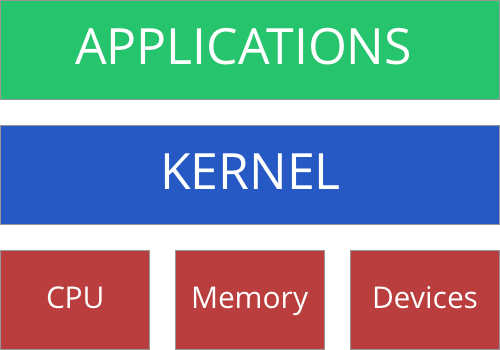
\includegraphics[width=3cm]{img/kernel}
    \caption{positie van kernel tussen de programma's en hardware}
    \label{fig:kernel}
\end{wrapfigure}

Als een programma wordt uitgevoerd dan bevindt die zich in de user space. Om het programma in werkelijkheid te kunnen uitvoeren moet toestemming gevraagd worden aan de kernel om de instructies van het programma realiseren. Deze instructies moeten worden nagegaan voor de veiligheid. Soms wordt er ook gesproken van memory isolation, waarbij de user space en kernel space niet rechtstreeks met elkaar kunnen communiceren. Dit is een veiligheidsmaatregel.

Volgend boek heeft meer informatie over de werking van de kernel (\cite{bovet_understanding_2005}).

De twee volgende delen, die hierop volgen, zullen de belangrijkste eigenschappen van unikernels uitleggen.

\section{Library besturingssysteem}

Elke virtuele machine binnen de architectuur van een productieomgeving heeft meestal één functie. Dit is al getoond in figuur \ref{fig:virtualmachine}. Elke guest heeft een gespecialiseerde rol om de middelen dat het ter beschikking krijgt optimaal te benutten.
Dezelfde architectuur en denkwijze van kan men terugvinden bij containers. De besturingssystemen die de virtuele machines en containers gebruiken is traditioneel te noemen. Dit is aangehaald in \cite{madhavapeddy_unikernels_2013}.

Als er dieper wordt ingegaan op deze evolutie dan kunnen we een patroon vaststellen: er worden steeds kleinere eenheden gebruikt. Eerst was de computer de eenheid, dan de virtuele machine en dan de software containers. Een unikernel kunnen we ook bekijken als een eenheid binnen dit patroon.

Het meest gebruikte besturingssysteem voor servers is het Ubuntu besturingssysteem (\cite{matthias_gelbmann_ubuntu_2016}) met 32\%. Veel programma's van databases tot en met web applicaties gebruiken het. Dit terwijl een database en een web applicatie andere middelen en functionaliteit nodig hebben.
Er zijn er ook gespecialiseerde besturingssystemen zoals Mini-OS (\cite{satya_popuri_tour_????}) die veel van de overbodige functies van een traditioneel besturingssysteem niet gebruiken. Deze gespecialiseerde besturingssystemen zijn in de minderheid en ook niet zeer gekend.

Traditionele besturingssystemen zijn niet de basis die men nodig heeft in een architectuur waar elke eenheid gespecialiseerd is. Alpine (\cite{alpine_linux_development_team_alpine_????}) is een Linux besturingssysteem dat een zeer minimale basis heeft. Tevens beschikt het over een uitgebreide package repository. Dit maakt het een ideaal besturingssysteem voor de basis van software containers. Je kan starten met een kleine basis en alle onderdelen toevoegen die je nodig hebt. Dit zorgt voor een container met een kleinere omvang. Hier wordt verder over uitgeweid in sectie \ref{sec:bene_unikernels}.

\begin{wrapfigure}{r}{0.4\textwidth}
    \centering
    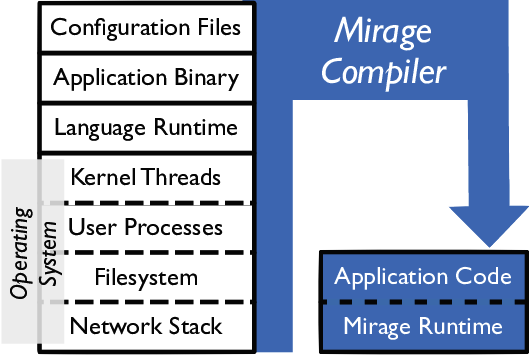
\includegraphics[width=6cm]{img/unikernel}
    \caption{algemeen besturingssysteem tegenover een unikernel implementatie \cite{madhavapeddy_unikernels_2013}}
    \label{fig:unikernel}
\end{wrapfigure}

Niet alleen hebben sommige delen geen nut meer, maar soms kan dat ervoor zorgen dat de prestatie van een besturingssysteem gehinderd wordt voor bepaalde taken. Het is dezelfde analogie als het gebruiken van een hamer voor elke klus.

Het concept van bibrary besturingssystemen (\cite{madhavapeddy_unikernels_2013}) neemt dit nog een stap verder. Er wordt met een absoluut minieme basis gestart. Daarna worden alleen de componenten toegevoegd die nodig zijn voor de functionaliteit die de eenheid uitvoerd. Library duidt op de verschillende onderdelen of componenten die kunnen worden toegevoegd.

Web applicaties hebben verschillende functies nodig om te kunnen communiceren. Hiervoor bestaan netwerkprotocollen. TCP is een kritiek protocol om te communiceren met het internet. Bij algemene besturingssystemen, zoals Ubuntu, is dit al aanwezig. Omdat er gestart wordt met een minimale basis, moeten deze protocollen geïmplementeerd worden. Gelukkig zijn er libraries die hiervoor kunnen gebruikt worden. De libraries, broncode en configuratie worden dan gecompileerd. Als resultaat heb je dan een image. Wanneer deze image wordt uitgevoerd dan hebben we een werkende unikernel. De unikernel wordt gecompileerd voor één omgeving en kan alleen gebruikt worden op die omgeving. Dit is een verschil met containers en virtuele machines die meer los staan van de omgeving waarin ze zich bevinden.

Er werd al gesproken dat de unikernel alleen zullen werken op de omgeving waarvoor het gecompileerd is. Dit is omdat de drivers voor de hardware componenten moeten worden geschreven. Kleine veranderingen in de specificatie of interface van een hardware component zorgt ervoor dat de driver niet meer werkt. Drivers zijn de grootste hindering die men tegenkomt bij library besturingssystemen. Hypervisors lossen dit probleem op door een standaard interface open te stellen. Zo moet er alleen maar één driver worden geschreven voor de hardware component. Dit neemt veel van het werk voor het maken van unikernels weg. De protocollen, waar eerder over gesproken is, wordt het grootste deel van het werk.

\section{Single Address Space}

In een unikernel bestaat er geen concept van user of kernel space. Alle processen bevinden zich binnen dezelfde omgeving. Dit zou problemen geven bij traditionele besturingssystemen. Maar bij het compileren van de unikernel wordt de broncode, libraries en configuratie gecontroleerd. Dit is om te kijken of er zich geen problemen kunnen voordoen. De afwezigheid van de communicatie tussen de kernel en user spaces zorgt voor een beter een prestatie. Deze verbetering van de prestatie komt ook doordat de hardware kan worden aangesproken zonder dat er verandert moet worden van context.

Eén globale address space zorgt voor problemen met de isolatie van processen. Meerdere programma's naast elkaar laten werken op een library besturingssysteem is complex. De hypervisor lost dit probleem gedeeltelijk op. Een mogelijke oplossing voor dit probleem wordt verder besproken in Hoofdstuk \ref{ch:microservices}.

\section{Veiligheid}

De hoge mate van veiligheid van unikernels is een gevolg van de specialisatie van de eenheid. Bij virtuele machines en containers zijn traditionele besturingssystemen de basis. Deze besturingssystemen hebben zeer veel functionaliteit dat niet nodig is voor de taak dat ze uitvoeren. De overbodige functionaliteit kan zorgen voor een lagere prestatie, maar ook voor meer veiligheidsrisico's. Het is gemakkelijker om de veiligheid te garanderen van een kleinere broncode tegenover een grote. Daar komt nog bij dat de unikernel implementaties gebruikt die specifiek zijn voor de omgeving. Het vraagt veel meer moeite om een gespecialiseerde implementatie te schrijven tegenover een algemene implementatie. Het marktaandeel van de algmene implementatie zal ook veel groter zijn tegenover de specifieke implementatie.

Verder heeft een unikernel geen shell of een andere mogelijkheid om een unikernel aan te passen terwijl hij aan het werken is. Eén unikernel overnemen heeft geen gevolg op de andere unikernels. Daarbij komt nog dat de hypervisors zelf meer veiligheid garanderen (\cite{colp_breaking_2011}).

\section{Andere voordelen}
\label{sec:bene_unikernels}

De omvang van een unikernel is kleiner dan een virtuele machine of een container. Zoals er al eerder werd aangehaald kunnen containers ook een kleine omvang hebben wanneer ze een miniem besturingssysteem gebruiken. Een voorbeeld daarvan is Alpine dat start vanaf 5 MB (\cite{_gliderlabs/docker-alpine_????}).
Een voorbeeld van de omvang van een unikernel kan gevonden worden in \cite[hoofdstuk 4, p.~10]{madhavapeddy_jitsu:_2015} met 1 MB.

Het systeem optimaliseren kan ook in veel grotere mate gebeuren (\cite{madhavapeddy_turning_2010}) dan traditioneel besturingssystemen.

\section{Productie}

Veel van de commentaar op unikernels komt van de moeilijkheden om te kijken wat er fout gaat in productie (\cite{bryan_cantrill_unikernels_2016}). Aanpassingen doen in productie om problemen te verhelpen is niet de beste manier om iets op te lossen. Het programma moet uitgebreid getest worden vooraleer het in de productieomgeving wordt opgesteld. Wanneer er dan toch iets fout gaat in productie dan zal men de situatie proberen na te bootsen in een soortgelijke omgeving. Het terugzetten van een oudere versie van het programma kan helpen om de gebruikers geen ongemak te laten ondervinden en tevens meer tijd te hebben om bepaalde problemen op te lossen.

\section{Hedendaags gebruik}

Unikernels kunnen momenteel gebruikt worden in beperkte situaties. Er was hetzelfde fenomeen te vinden bij software containers een paar jaar geleden vooraleer Docker op de voorgrond trad. Elke technologie ondergaat een tijd om matuur te worden.

In het volgende deel zullen we implementaties van unikernels vergelijken om een beter beeld te krijgen van de huidige mogelijkheden en het huidige landschap binnen unikernels.

\chapter{Vergelijking implementaties unikernels}

\section{Inleiding}

In het hoofdstuk over unikernels zijn er een aantal voorbeelden van moderne implemenaties van unikernels aangehaald. In dit hoofdstuk zullen er een aantal implementaties van unikernels worden vergeleken met elkaar. Het volgende deel zal aanhalen welke criteria er zullen gebruikt worden om deze vergelijking te realiseren.

\section{Criteria}

\begin{description}
\item [Implementatie programmeertaal]
Op het eerste zicht lijkt de programmeertaal waarin de implementatie geschreven is niet belangrijk. Dit is wel belangrijk voor te weten of het een programmeertaal is waarbij gemakkelijk kan gewerkt worden.
Een meer voor de hand liggende programmeertaal, zoals C++, zal gemakkelijker open source ontwikkelaars aantrekken. En dat is ook een belangrijk gegeven.
De meeste implementaties zijn in C/C++ geschreven. Dit komt vooral door het feit dat veel software ontwikkelaars die zich bezig houden met unikernels komen vanuit een achtergrond met besturingssystemen komen.
De meest gebruikte programmeertaal voor een besturingssysteem is C/C++.

\item [Hypervisors] 
Hypervisors zijn een groot deel van de keuze voor het kiezen van een implemenatie. De meest gebruikte unikernels zijn beschikbaar op een aantal hypervisors. Als er veel omgevingen waarop de unikernels kunnen werken dan is het gemakkelijk om van omgeving te veranderen als bedrijf. Wendbaarheid en inspelen op veranderingen zal gemakkelijker gebeuren wanneer je beschikt over een uitgebreid aantal mogelijkheden.

\item [Ondersteunde programmeertalen]
Sommige unikernels ondersteunen een aantal programmeertalen om te zorgen dat er niet moet veranderd worden van implementatiem, wanneer je een andere programmeertaal kiest voor een bepaalde toepassing.
Programmeertalen hebben hun sterke en zwakke kanten en keuze hebben uit een aantal programmeertalen helpt voor een groter aantal verschillende toepassingen te schrijven.

\item [GitHub stars] 
GitHub bepaalt de status van jouw open source project. Open source software wordt meer en meer gebruikt door bedrijven en de keuze is gemakkelijk te maken tussen een project met veel sterren en een project met weinig sterren. Hierbij spreken we wel over projecten met dezelfde functionailiteit. Door GitHub kan gekeken worden of er actief aan het project gewerkt word of het onderhouden wordt. De gemeenschap van een project is ook belangrijk voor de keuze te maken van welk project je kiest.

\end{description}

\begin{table}[ht]
\caption{Implementaties unikernels}
\begin{center}
    \begin{tabular}{| l | l | l | l | l |}
    \hline
    Naam & Taal implementatie & Hypervisor & Ondersteunde talen & GitHub sterren \\ \hline
    ClickOS & C/C++ & Xen & bindings & 243 \\ \hline
    HaLVM & Haskell & Xen & Haskell & 665 \\ \hline
    LING & C/Erlang & Xen & Erlang & 523 \\ \hline
    Rumprun & C & hw, Xen, POSIX & C, C++, Erlang, Go, ... & 469 \\ \hline
    MirageOS & OCaml & Xen & OCaml & 657 \\ \hline
    IncludeOS & C++ & KVM, VirtualBox & C++ & 1341 \\ \hline
    OSv & C/C++ & KVM, Xen, ... & JVM & 2121 \\ \hline
    \end{tabular}
\end{center} 
}
\label{tab:impl_unikernels}
\end{table}

De inhoud van de bovenstaande tabel wordt per implementatie uitgelegd in het volgende deel.

\newpage

\section{Implementaties van moderne unikernels}

\subsection{ClickOS}
\begin{description}
  \item [Implementatie programmeertaal]: C/C++
  \item [Hypervisors]: Xen
  \item [Ondersteunde programmeertaal]: ondersteund door bindings
  \item [GitHub stars]: 243
\end{description}

ClickOS  (\cite{martins_clickos_2014}) wordt ontwikkeld door Cloud Networking Performance Lab.

De toepassingen, waarvoor ClickOS voornamelijk wordt gebruikt, zijn middleboxes. De programma's waarvoor ClickOS wordt voor gebruikt zijn middleboxes. Een middlebox is een netwerk applicatie dat netwerktrafiek kan omzetten, filteren, inspecteren of manipuleren. Voorbeelden hiervan zijn firewalls en load balanceres.
Een modulaire router vormt het startpunt. Op deze router worden onderdelen toegevoegd. Deze unikernel werkt alleen op MiniOS. MiniOS is beschikbaar bij de broncode van de Xen hypervisor.

Door een evolutie binnen netwerk laag (\cite{garcia_villalba_trends_2015}) wordt veel van de functionaliteit, die vroeger bij de hardware zat, nu in software geïmplementeerd. Dit laat toe om een eigen implementatie schrijven om veel functionaliteit van de hardware over te nemen.
Dit zorgt voor een implementatie die aangepast kan worden aan de eigen situatie.

De use cases waarbinnen ClickOS kan gebruikt worden zijn beperkt. Als je geen gebruik wilt maken van ingebouwde netwerk functionaliteit van de hardware dan is ClickOS de uitgesproken keuze.

Er wordt Swig gebruikt om ondersteuning te bieden voor hogere programmeertalen. Swig maakt een bindings die C/C++ verbindt met een hogere programmeertaal.

ClickOS verwijst naar zijn packages als elements. Die elements voeren in bepaalde actie uit. Dit zijn hele kleine stukken functionaliteit. Er zijn om en bij de 300 elementen beschikbaar voor te gebruiken. Het is simpel om zelf je eigen element te maken en te distribueren.

Meer informatie kan gevonden worden volgende website: \cite{cloud_networking_performance_lab_cloud_????}.

\subsection{HaLVM}

\begin{description}
  \item [Implementatie programmeertaal]: Haskell
  \item [Hypervisors]: Xen
  \item [Ondersteunde programmeertaal]: Haskell
  \item [GitHub stars]: 665
\end{description}

HaLVM (\cite{galois_inc._haskell_????}) wordt ontwikkeld door Galios. Galios is een software ontwikkelings agentschap dat unikernels al een tijd in productie gebruikt.
Er zijn niet veel bedrijven die unikernels al gebruiken in productie, dus ze hebben al ervaring met de mogelijkheden en moeilijkheden van unikernels.

De programmeertaal waarin de unikernel van HaLVM wordt geschreven is Haskell. Haskell is een functionele programmeertaal met een uitgebreid type system. HaLVM is een implementatie die één supervisor en één programmeertaal ondersteund.

Het werd ontwikkeld met als doel voor besturingssysteem componenten snel te maken en te testen. Na een tijd is het geëvolueerd naar andere use cases.

Bij HalVM wordt de Xen hypervisor als omgeving gebruiken. Er is een integratie met de Xen hypervisor waarop de core library van HaLVM op rust. Er bestaat ook een communications library die bestaat uit het Haskell File System en de Haskell Network Stack. Deze library kan gebruikt worden in de meeste gevallen als je een netwerkfunctionaliteit nodig hebt. Als we meer mogelijkheden nodig hebben voor een programma dan kunnen er modules worden toegevoegd. Er is een ecosysteem uitgebouwd om het gemakkelijker te maken voor software ontwikkelaars om hun eigen modules te bouwen.

De werkwijze is de volgende: eerst wordt er zoveel mogelijk functionaliteit als een normaal Haskell programman geschreven. Daarna moet het programma aangepast worden om het te gebruiken op HaLVM.
Dit is niet gemakkelijk bij uitgebreide applicaties zijn, want er zijn maar beperkte mogelijkheden om te debuggen op HalVM.

Zoals in de meeste gevallen moet de compiler van Haskell worden aangepast om de unikernel te maken. Het is ook geen probleem om standaard Haskell libraries in de code te gebruiken.

Het wordt gebruikt door Galios in productie en dit maakt het gemakkelijk om vragen te stellen. De GitHub repository, waar de applicatie zich op bevindt, is over het algemeen actief en is populair voor maar één programmeertaal te ondersteunen.

\subsection{Ling}

\begin{description}
  \item [Implementatie programmeertaal]: C/Erlang
  \item [Hypervisors]: Xen
  \item [Ondersteunde programmeertaal]: Erlang
  \item [GitHub stars]: 523
\end{description}

Ling (\cite{erlang_on_xen_cloudozer/ling_????}) is een Erlang virtuele machine die werkt op de Xen hypervisor. Het bedrijf achter Ling is Cloudozer. Ze hebben al meerdere language runtimes gemaakt die rechtstreeks op Xen werken.
Ling is open source maar de andere tools, die onder meer het beheren doen van unikernels, zijn niet open source. Wanneer je problemen met het ecosysteem hebt, moet de ondersteuning van Cloudozer gecontacteerd worden.

Zoals bij HaLVM moet eerst de applicatie geschreven worden in Erlang. De package manager die gebruikt word met Erlang is Rebar, dit is de standaard Erlang package manager. Na het omzetten van de applicatie naar een Xen afbeelding zou de unikernel moeten werken.

Railing is een tool die meegeleverd is met Ling die je toelaat om erlang on Xen afbeeldingen te maken. We gebruiken ook xl utility van Xen om domeinen te beheren.
De focus van Erlang on Xen was de Xen hypervisor in het begin. 

Bij het uitbrengen van een nieuwe versie van LING is het mogelijk geworden om ports te maken voor andere omgevingen. Dit heeft veel nieuwe omgevingen, zoals IOT en mobiele omgevingen, mogelijk gemaakt.
Unikernel kunnen handig zijn op deze omgevingen omwille van de kleine omvang, er is namelijk geen uitgebreid besturingssysteem nodig. 

Verder opent dit ook de mogelijkheid voor de unikernels van LING op bare-metal te laten werken.

\subsection{Rumprun}

\begin{description}
  \item [Implementatie programmeertaal]: C
  \item [Hypervisors]: hardware, Xen, KVM
  \item [Ondersteunde programmeertaal]: onder meer C, C++, Erlang, Go, Javascipt, Python, Ruby
  \item [GitHub stars]: 469
\end{description}

Rumprun  (\cite{rumpkernel/rumprun_0000}) gebruikt rump kernels voor hun implementatie. Deze rump kernels worden samengesteld uit componenten afkomstig van NetBSD. NetBSD is een traditioneel besturingssysteem maar is modulair geschreven. Men kan het dus gebruiken om een rump kernel samen te stellen.

Er is een uitgebreide keuze aan hypervisors waaruit je kan kiezen. De term hw duidt op hardware. Dit betekent dat rumprun één van de enige implementaties is die rechtstreeks kan werken op hardware. De unikernel kan ook werken op besturingssystemen die een POSIX-interface hebben. De POSIX-interface duidt op Unix systemen.

Er zijn verschillende soorten unikernels. Sommige unikernels specialiseren op basis van programmeertaal en andere op basis van omgeving. Sommige doen zelf beide. Rumprun doet beide. Dit is wel niet zonder gevolg. De prestatie zal niet een gespecialiseerde unikernel kunnen evenaren.

De rump-run packages zijn implementaties van drivers, protocollen en libraries die kunnen toegevoegd worden aan de rumprun kernels. Er zijn een groot aantal packages die kunnen gebruikt en de meest bekende zijn aanwezig.
Het spijtige is wel dat er nog geen packaging systeem aanwezig is. Dit zou er wel voor zorgen dat er gewerkt kan worden met verschillende dependencies en versies van packages.

Rumprun verziet zelf geen compiler. Er wordt gebruik gemaakt van een compiler die aanwezig is op het systeem. In het geval van Mac OS X moet je een aparte compiler installeren.

De programmeertalen die ondersteund zijn, zijn de volgende: C, C++, Erlang, Go, Javascript(node.js), Python, Ruby en Rust. De keuze van programmeertalen is uitgebreid.

Meer informatie is te vinden in volgende thesis: \cite{kantee_flexible_2012}.

\subsection{MirageOS}

\begin{description}
  \item [Implementatie programmeertaal]: OCaml
  \item [Hypervisors]: Xen, Unix
  \item [Ondersteunde programmeertaal]: OCaml
  \item [GitHub stars]: 657
\end{description}

Er kan gezegd worden dat het voor een deel allemaal begon bij MirageOS (\cite{mirage/mirage_0000}). Hun paper (\cite{madhavapeddy_unikernels_2013}) over unikernels en MirageOS wakkerde veel interesse aan rond unikernels. Ervoor was er wel al sprake van unikernels maar MirageOS zorgde voor veel nieuwe initiatieven.

Mirage is een cloud besturingssysteem gemaakt om veilige netwerk toepassingen met een hoge prestatie te maken op verschillende omgevingen.

De programmeertaal dat gebruikt word voor een MirageOS applicatie te maken is OCaml.
OCaml is de algemene implementatie van de Caml programmeertaal en voegt object georiënteerd programmeren toe. Het wordt extensief gebruikt door facebook. Deze taal is niet heel erg bekend en dit kan ervoor zorgen dat het niet veel tractie heeft.

De voornaamste redenen om OCaml te gebruiken zijn static type checking en automatic memory management. De eerste reden is om tegen te gaan dat er iets fout gaat wanneer een programma aan het werken is. De compiler gaat kijken of hij geen onveilige code kan vinden. Als dit het geval is, wordt het programma niet gecompileerd.
Memory management is belangrijk voor resource leaks tegen te gaan. Resource leaks kunnen ervoor zorgen dat het programma meer resources gebruikt dan nodig is. In het extreme geval kan het systeem waarop het programma werkt ook hinder ondervinden van dit probleem.

De applicatie kan geschreven worden op een Linux of Mac OSX besturingssysteem. Deze applicatie kan dan werken op een Xen of Unix omgeving. Dit geeft veel mogelijkheden op het vlak van omgevingen. Er zijn plannen om mobiele omgevingen te ondersteunen.

MirageOS bestaat al een tijd en heeft een groot aantal libraries ter beschikking. Het heeft een uitstekende toolchain voor het compileren van programma's en het debuggen van de resulterende unikernel. Debuggen kan soms tot problemen leiden bij unikernels want er kan niet in de unikernel gekeken worden welke problemen zich voordoen. Dit komt omdat de unikernel geen shell heeft. De debug optie kan hierbij helpen.

\subsection{IncludeOS}
\begin{description}
  \item [Implementatie programmeertaal]: C/C++
  \item [Hypervisors]: KVM, VirtualBox
  \item [Ondersteunde programmeertaal]: C++
  \item [GitHub stars]: 1341
\end{description}

IncludeOS (\cite{oslo_and_akershus_university_college_hioa-cs/includeos_????}) is gemotiveerd door het paper van \cite{bratterud_maximizing_2013}. Het onderscheid tussen een minimale virtuele machine tegenover een unikernel is zeer klein. Daarom worden beide termen afwisselend gebruikt. Net zoals ClickOS moeten de applicaties geschreven worden in C++.

IncludeOS zorgt voor een bootloader, standaard libraries, modules voor de drivers te implementeren en een build- en deploysysteem. Het is simpel om applicaties te maken voor deze unikernel. Je moet allen één dependency toevoegen aan het programma. Dan kan het worden omgezet naar een unikernel. Er veranderd dus niet veel voor de software ontwikkelaars. Dit zorgt voor een vlotte overgang en dit is zeker belangrijk wanneer men kiest voor minimale applicaties te maken.

Meerdere processen tegelijk laten werken op een unikernel van includeOS is niet mogelijk. Dit kan sommige software ontwikkelaars afschrikken. Het gebruik van microservices (hoofdstuk \ref{ch:microservices}) is nog niet wijdverspreid en kan een factor zijn bij het selecteren van een unikernel implementatie. Enerzijds gaan bedrijven nooit bij unikernels komen wanneer hun architectuur niet gebaseerd op microservices. Er zijn ook geen race conditions mogelijk omdat er maar één proces mogelijk is.

Momenteel ligt de focus van IncludeOS voornamelijk op C++. Dit is een strategie dat kan helpen wanneer software ontwikkelaars zoeken naar een implementatie die een gemeenschap heeft. IncludeOS heeft een grote gemeenschap van C++ software ontwikkelaars. Hun doel is vooral om een soortgelijk Node.js te maken maar dan in efficiënt C++.

Er zijn geen plannen om hogere programmeertalen zoals Javascript te ondersteunen. Ook is IncludeOS niet POSIX compliant en dit kan voor problemen zorgen wanneer er extra functionaliteit moet worden toegevoegd.

Als omgeving focussen ze KVM en virtualbox. Het is het dus gemakkelijk om een unikernel te testen op de ontwikkelomgeving. Als je services schrijft in C++ dan is IncludeOS een zeer goede keuze. Er kan meer informatie gevonden worden op de GitHub repository: \cite{oslo_and_akershus_university_college_hioa-cs/includeos_????}.

\subsection{OSv}

\begin{description}
  \item [Implementatie programmeertaal]: C/C++
  \item [Hypervisors]: VMWare, VirtualBox, KVM, Xen
  \item [Ondersteunde programmeertaal]: Java
  \item [GitHub stars]: 2121
\end{description}

OSv (\cite{cloudius-systems/osv_0000}) is een implementatie die een grote naam heeft binnen de unikernel wereld. De meest uitgebreide unikernel vanuit mijn oogpunt is OSv. Er wordt een hoog aantal programmeertalen geondersteund. Waaronder Java, Ruby, Javascript, Scala en vele anderen. Hierbij moeten wel wel vermelden dat de implementaties van Ruby en Javascript in Java zijn geschreven. Rhino en JRuby zijn de namen van deze implemenaties. Het is simpel om deze programmeertalen toe te voegen wanneer je Java als programmeertaal ondersteunt. Er wordt gewerkt om de native ondersteuning voor deze programmeertaal te gebruiken.

Verder kunnen de resulterende unikernels werken op veel omgevingen: VMware, VirtualBox, KVM en Xen. Het is een indrukwekkende lijst van hypervisors de je kan gebruiken. Dit kan helpen om tegen te gaan dat men vast zou zitten op een bepaalde omgevingen.

Zoals IncludeOS voorheen is OSv geschreven in C++.

Voor het beheren van een OSv instance kan gebruik worden gemaakt van de GUI. Bij de meerderheid van unikernels is informatie te vinden door middel van een GUI onmogelijk. Extensies met de hypervisor kunnen hierbij helpen, maar dan nog laat de UX de wensen over. De GUI is gebouwd op een REST API die de componenten van OSv openstellen. Dit komt overheen met de manier hoe Docker hun architectuur werkt. Deze componenten stellen een API open waar de tools verder opgebouwd kunnen worden. Er is een API-specificatie die kan bekeken worden om te zien hoe deze componenten met elkaar werken.

OSv ondersteund Amazon Web Services en Google Container Engine als cloud providers. Het is uitzonderlijk dat een unikernel zoveel informatie heeft over hoe het moet gebruikt worden. Er is documentatie over cloud providers, hypervisors, hoe OSv moet gebruikt worden, hoe programma's moet omgezet naar de implementatie. En wat nodig is om zelf te sleutelen aan OSv.

Het is de meest populaire implemenatie van unikernels van alle implementaties die we hebben overlopen tijdens deze vergelijking. Ook de activiteit op de Github repository is het hoogste van alle bekeken unikernels.

Meer informatie is te vinden in volgende paper: \cite{kivity_osvoptimizing_2014}.

\section{Conclusie}

Er zijn veel verschillende soorten implementaties van unikernels op dit moment. Er is MirageOS die als één van de eerste opkwam en ook de meest extreme weg opgaat met het starten van een minieme basis. HalVM bevindt zich in aan de dezelfde kant als MirageOS. Terwijl OSv en Rumprun zich bevinden aan de overkant. Ze ondersteunen een groot aantal programmeertalen en omgevingen. Dit wordt mogelijk gemaakt door een compatibiliteitslaag te gebruiken. 

Hetzelfde fenomeen kunnen we vinden met de toepassingen waar de unikernels kunnen voor gebruikt worden. ClickOS heeft vooral middlebox applicaties als doel en andere unikernels kunnen voor uiteenlopende situaties kunnen gebruikt worden.

Volgend hoofdstukken zullen bekijken welke technologiën en denkwijzes naar de voorgrond komen bij unikernels.

\chapter{Unikernels in de praktijk}
\label{ch:unikernels_praktijk}

\section{Inleiding}

Nadat het theoretische gedeelte is uitgelegd, en een vergelijking van de verschillende soorten implementaties van unikernels is uitgevoerd, wordt het tijd om unikernels uit te testen in de praktijk. De huidige implementaties van unikernels geven een zekere vrijheid wat voor soort applicaties er kunnen opgezet worden. 

Er kan gesproken worden over twee types van applicaties: dynamische en statische. Hiernaar wordt ook verwezen in het Engels als stateless en statefull. Blogs en websites zonder veel functionaliteit zijn stateless. Het resultaat van de applicatie qua functionaliteit zal hetzelfde zijn voor iedereen. Statefull applicaties zijn web applicaties zoals Wordpress en de meeste applicaties waar er informatie wordt bijgehouden en kan worden aangepast zonder de applicatie aan te passen en herop te starten. Het overgrote deel van de applicaties die werken met unikernels zijn stateless.

Veel van toepassingen die werken met unikernels bevinden zich meestal in een bepaald segment. Dit is het geval met technologiëen die nog moet toegroeien naar algemene of meerdere use cases. Toepassingen die gebruikmaken van unikernels maken zullen zich grotendeels bevinden binnen de netwerklaag. Bij de algemenere implementaties van unikernels die zich gaan focussen om meerdere programmeertalen is een applicatie zoals wordpress gemakkelijker op te stellen. Rumprun heeft al pogingen gedaan om een soort van RAMP (RumpRun, Apache, MySQL, PHP) opstellingen te maken maar dit staat nog in vroeg stadium. Het maken van unikernels voor statische applicaties is dus een betere keuze voor de verschillende soorten unikernels te vergelijken. Hierdoor werd gekozen voor het opzetten van een unikernel voor een statische blog.

MirageOS is een unikernel die zich focust op OCaml. Het bestaat al een geruime tijd en heeft al een grote groep achter hen staan. Als algemene unikernel is er de keuze tussen RumpRun en OSv. Rumprun is de meest mature optie van de twee en er is de meeste informatie over beschikbaar op het huidig moment.

Als hypervisor wordt er gekozen voor Xen want MirageOS en Rumprun ondersteunen deze beide. Bij nader onderzoek is gebleken dat Xen de meest stabiele omgeving is om de unikernels op te testen. Bij het gebruiken van een Unix omgeving werden er veel obstakels gevonden die niet op een korte termijn waren op te lossen. De meeste demo's van unikernels worden ook meestal op de Xen omgeving gedaan omwille van de grote van het marktaandeel van Xen.

\section{Opstelling}

Deze opstelling wordt uitgevoerd op een virtuele machine want er worden extensieve veranderingen uitgevoerd op het besturingssysteem. Voor deze opstelling lokaal op te stellen zijn er drie vereisten nodig. Ten eerste de Virtualbox hypervisor voor een virtuele machine op te laten werken. Verder Vagrant om de ontwikkelingomgeving op te stellen. Vagrant en Virtualbox gaan hand in hand om een simpele start te hebben wanneer een bepaalde ontwikkelingomgeving nodig hebt. Vagrant werkt door middel van een bestand (VagrantFile) met alle configuratie erin beschreven. Het haalt eerst een box op waarop de configuratie wordt toegepast. Een box kan een Ubuntu besturingssysteem dat nog niet is aangepast of in deze situatie een besturingssysteem waarop allerhande configuraties zijn uitgevoerd. Packer is de laatste vereiste, het zal gebruikt worden om de box op te stellen die zal gebruikt worden. 

\begin{description}
\item [Virtualbox] - https://www.virtualbox.org/
\item [Vagrant] - https://www.vagrantup.com/
\item [Packer] - https://www.packer.io/ 
\end{description}

Allereest moeten alle voorgenoemde vereisten zijn geïnstalleerd op uw machine voor er verder kan worden gegaan. MirageOS heeft een repository met alle benodigdheden om deze virtuele machine op te stellen. Deze kan gevonden worden op de volgende link: https://github.com/michieldewilde/mirage-vagrant-vms. Haal deze repository lokaal op de machine en navigeer naar de locatie van deze opgehaalde folder. Er is keuze uit ubuntu 14.04, ubuntu 14.10, debian 7.8.0 en xenserver 6.5.0. Er is gekozen voor Ubuntu 14.04 omdat er het minste problemen bij dit besturingssysteem zijn vastgesteld voor deze opstelling. De Makefile bevat voor de gemakkelijkheid commando's voor de virtuele machine op te stellen zonder een lijst van commando's in te geven.

\noindent Het volgende commando zal een nieuwe box aanmaken door het gebruik van Packer:
\begin{lstlisting}[language=bash]
  $ make ubuntu-14.04-box
\end{lstlisting}

\noindent Het volgende commando neemt de box, die is aangemaakt door het vorige commando, en past de configuratie erop toe:
\begin{lstlisting}[language=bash]
  $ make ubuntu-14.04-box
\end{lstlisting}

\noindent Navigeer naar de folder van het gekozen besturingssysteem en ssh in de virtuele machine: 
\begin{lstlisting}[language=bash]
  $ cd ubuntu-14.04 && vagrant ssh
\end{lstlisting}

\section{MirageOS}

MirageOS is gestart vanaf nul met een schone lei. Dit betekende dat veel van de bestaande tools die nu worden gebruikt worden, zoals webservers (Apache, Nginx) en Databases (MySQL), herschreven zouden moeten worden. Het duurt een tijd voordat deze tervoorschijn komen en dit is één van de grootste redenen dat er gekozen is voor een statische applicatie.

De opstelling die gemaakt is in de vorige sectie heeft de toolset van MirageOS ook geïnstalleerd. Verder moet er worden gekeken of de juiste versie van Ocaml en OPAM (package manager) is geïnstalleerd:

\noindent OPAM versie:
\begin{lstlisting}[language=bash]
  $ opam --version
  # De versie moet minstens 1.2.2 zijn.
  1.2.2
\end{lstlisting}

\noindent Ocaml versie:
\begin{lstlisting}[language=bash]
  $ ocaml -version
  # Deze moet 4.02.3 of hoger zijn.
  $ opam switch 4.02.3
\end{lstlisting}

In de login shell moet de omgeving van opam geëvalueerd wanneer er ingelogd wordt. Dit kan gedaan worden door de volgenden lijn toe te voegen aan het ~/.bashrc bestand:

\begin{lstlisting}[language=bash]
  $ eval `opam config env`
\end{lstlisting}

\noindent Verder moeten er ook gekeken of de versie van mirage niet moet upgedate moet worden:
\begin{lstlisting}[language=bash]
  $ opam install mirage
  $ mirage --help
  # Versienummer moet hoger zijn 2.9.0
\end{lstlisting}

Het mirage commando kan gebruikt worden voor applicaties te maken en te deployeren.

Als statische website zullen we de website van MirageOS zelf gebruiken. De repository van de website bevindt zich op de volgende link: https://github.com/mirage/mirage-www/. Eerst moet de repository in de virtuele machine worden gehaald. 

\noindent Dit doen we door het git commando te gebruiken:
\begin{lstlisting}[language=bash]
  $ git clone https://github.com/mirage/mirage-www/
\end{lstlisting}

Vooraleer we de omgeving van de applicatie gaan configureren moet het mogelijk worden gemaakt om de Xen hypervisor te laten communiceren met de virtuele machine. Deze twee zijn afgeschermd van elkaar en daarom moet er een TUN/TAP constructie worden gemaakt. 

sudo modprobe tun
\noindent Dit doen we als volgt:
\begin{lstlisting}[language=bash]
  $ sudo apt-get install tunctl
  $ sudo modprobe tun # laden van de tuntap kernel module
  $ sudo tunctl # maak een tap0 interface
  $ sudo ifconfig tap0 10.0.0.1 up # start tap0 op en wijs tap0 naar IP
\end{lstlisting}

Navigeer naar de gehaalde folder van de MirageOS website. 
\noindent Daarna moet de omgeving voor de applicatie worden ingesteld:
\begin{lstlisting}[language=bash]
  $ cd mirage-www
  $ make prepare
  $ cd src
  $ mirage configure --xen \ # configureren voor de Xen hypervisor
      -vv --net direct \ #  direct MirageOS network stack
      --dhcp true \ maak gebruik van DHCP
      --tls false --network=0
\end{lstlisting}

Hierdoor is de omgeving van de applicatie goed ingesteld.
\noindent Het compilen van de unikernel:
\begin{lstlisting}[language=bash]
  $ make
\end{lstlisting}

Eerst moeten nog file blocks worden aanmaken om de afbeeldingen en de stylesheets te kunnen gebruiken:
\noindent Aanmaken file blocks
\begin{lstlisting}[language=bash]
  $ ./make-fat_block1-image.sh
\end{lstlisting}

Verder moet er nog een paar wijzigingen worden aangebracht in het www.xl bestand. Dit bestand wordt doorgegeven naar de Xen launcher om de unikernel te starten.
\noindent Het disk gedeelte moeten worden aangepast naar het volgende:
\begin{lstlisting}
disk = ['format=raw,
         vdev=xvde,
         access=rw,
         target=/home/vagrant/mirage-www/src/fat_block2.img',
        'format=raw,
         vdev=xvdc,
         access=rw,
         target=/home/vagrant/mirage-www/src/fat_block1.img
      ']
\end{lstlisting}


\noindent Uiteindelijk kunnen we de unikernel starten:
\begin{lstlisting}[language=bash]
  $ sudo xl -v create -c www.xl
\end{lstlisting}

Doorheen de output kan gezien worden op welk IP de statische website staat te luisteren. Als er gegaan wordt naar dat IP om de lokale machine dan kan de MirageOS website worden gezien.

\section{Rumprun}

Bij de rumprun unikernel zal gebruik gemaakt worden van Nginx webserver om een statische website weer te geven. 
Allereerst moeten we de build tools van Rumprun installeren.
Dit wordt gedaan als volgt.

\noindent We halen de Rumprun repository op en alle dependencies
\begin{lstlisting}[language=bash]
  $ git clone http://repo.rumpkernel.org/rumprun
  $ cd rumprun
  $ git submodule update --init
\end{lstlisting}

Verder moeten we toolchain maken voor de omgeving dat zal gebruikt worden. In dit geval is het Xen.
\begin{lstlisting}[language=bash]
  $ ./build-rr.sh xen
\end{lstlisting}

Dit maakt een folder aan genaamd rumprun met daarin een bin folder dit moet toegevoegd worden aan het PATH.
\noindent Toevoegen Rumprun toolchain aan PATH:
\begin{lstlisting}[language=bash]
  $ export PATH=${PATH}:$(pwd)/rumprun/bin
\end{lstlisting}

De toolchain voor Rumprun unikernels te maken is geïnstalleerd en nu moet er een nginx Rumprun unikernel worden opgehaald.
\noindent Ophalen Nginx unikernel:
\begin{lstlisting}[language=bash]
  $ git clone http://repo.rumpkernel.org/rumprun-packages
  $ cd rumprun-packages/
  $ cd nginx/
\end{lstlisting}

Er moet ook een package worden geïnstalleerd om een ISO bestand te maken. Dit zal gebruikt worden voor bestanden te laden in de unikernel.
\noindent Installeren genisoimage:
\begin{lstlisting}[language=bash]
  $ sudo apt-get install genisoimage
\end{lstlisting}

De volgende stap is om Nginx te compileren.
\noindent Compileren Nginx:
\begin{lstlisting}[language=bash]
  $ make
\end{lstlisting}

De unikernel werkt nu al maar moet omgezet worden naar een unikernel die werkt op de Xen hypervisor.
\noindent unikernel voor Xen maken:
\begin{lstlisting}[language=bash]
  $ rumprun-bake xen_pv ./nginx.bin bin/nginx
\end{lstlisting}

Hierbij is nginx.bin de unikernel die moet worden gestart.

\noindent Uitvoeren van de Nginx unikernel:
\begin{lstlisting}[language=bash]
  $ rumprun -T tmp xen -M 64 -i \
  $ -b images/data.iso,/data \ # data van www folder laden (inhoud van statische website)
  $ -I mynet,xenif,bridge=br0 -W mynet,inet,dhcp \ # dhcp instellen
  $ -- nginx.bin -c /data/conf/nginx.conf # laden van unikernel en configuratie
\end{lstlisting}

Het IP van de Nginx webserver is te vinden in de output in het gedeelte van DHCP. Het is het IP adres.

De bridge br0 ,die in MirageOS en Rumprun unikernel wordt gebruikt, is een host-only bridge tussen de host en de virtuele machine om netwerkverkeer tussen beide te laten werken.

\section{Conclussie}

Dit hoofdstuk focust vooral op de tools dat moeten gebruikt worden om de unikernels te maken en te deployen. Elke implementatie van een unikernel heeft zijn eigen build tools en meestal zijn deze niet echt consistent met elkaar. Dit kan leiden tot frustaties als er naar andere omgeving wordt verhuisd en er gebruikt van andere build tools moet worden gemaakt. Er zijn verschillende pogingen om al deze build tools achter één interface te brengen en ze zo simpel te kunnne gebruiken. Spijtig genoeg staat dit alles nog in een vroeg stadium. Statische applicaties en specifieke netwerktoepassingen zijn één van de enige mogelijkheden momenteel om unikernels in productie te gebruiken. Er is ook geprobeerd geweest om een Wordpress blog op te stellen met behulp van Rumprun maar er werd zodanig veel tegen moeilijkheden gestoten dat dit zeer moeilijk was. Daarbij kwam nog dat het hele gegeven zeer traag is om te veranderingen te kunnen maken en de gevolgen ervan te zien. In de volgende hoofdstukken zal er gekeken worden naar concepten die essentieëel zijn binnen een architectuur die gebruik maakt van unikernels.

\chapter{Microservices}
\label{ch:microservices}

De meeste programma's worden gemaakt door een monolothische architectuur te hanteren (\cite{villamizar_evaluating_2015}). Alle functionaliteit en verantwoordelijkheden worden gestopt in één programma. Dit soort van programma wordt een monoliet of monolith in het Engels genoemd. De architectuur waarin deze soort programma's voorkomen noemen we een monolithische architectuur. Software ontwikkelaars worden geleerd door middel van patronen (\cite{tichy_catalogue_1997}) om functionaliteit en verantwoordelijkheid van elkaar te scheiden. Modulariteit is hierbij een belangrijk gegeven.

\begin{wrapfigure}{r}{0.4\textwidth}
    \centering
    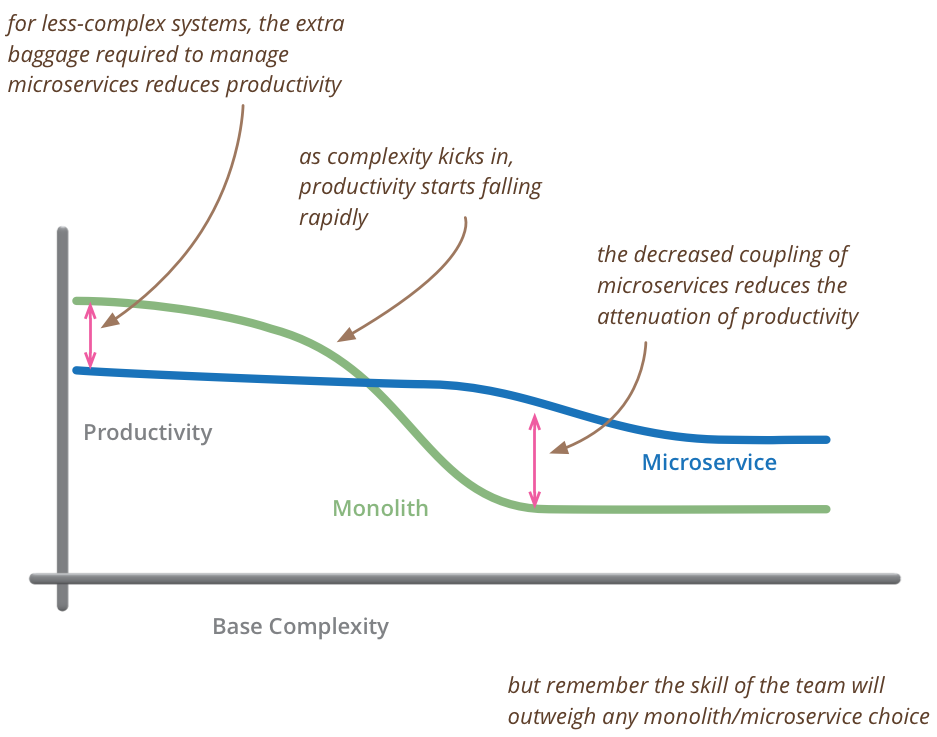
\includegraphics[width=6cm]{img/microservices_monolith}
    \caption{Productiviteit en complexiteit van microservices architectuur tegenover een monolithische architectuur (\cite{martin_fowler_microservicepremium_2015})}
    \label{fig:pr}
\end{wrapfigure}

Een probleem dat veel voorkomt bij een monolithische architectuur is dat het programma zeer complex wordt na verloop van tijd (\cite{villamizar_evaluating_2015}). Functionaliteit toevoegen is niet vanzelfsprekend bij een complex programma want er moet rekening worden gehouden met de andere delen van het programma. Nieuwe software ontwikkelaars die het programma niet kennen moeten eerst een paar weken het programma verkennen. Dan pas kan er begonnen worden met nieuwe functionaliteit te schrijven.

Schaalbaarheid is een probleem waar ook tegen gelopen wordt na verloop van tijd (\cite{villamizar_evaluating_2015}). Sommige onderdelen van een programma moeten meer trafiek kunnen verwerken dan andere delen. Zoals we al aanhaalden in hoofdstuk \ref{ch:virtualisatie}, hebben verschillende soorten programma's nu éénmaal andere middelen nodig. Dit is hetzelfde bij de interne delen van programma. Het schalen van deze componenten is alleen mogelijk door een nieuwe instantie toe te voegen van de hele applicatie of de implementatie te verbeteren. Eén groot programma is ook niet handig voor grote teams te laten samenwerken. Het uitbrengen van een versie moet dan nagegaan worden bij alle teams die aan dat programma werken.

Al langer bestaat het idee om een groot programma op te splitsen in kleinere programma's. Telecommunicatie is een industrie waarin microservices al werden gebruikt \cite{griffin_survey_2007}. De opkomst van containers heeft dit deze werkwijze meer verspreid. Dit komt omdat het gemakkelijker is geworden om kleinere programma's met elkaar te verbinden zelf als ze zich niet op dezelfde omgeving bevinden. De architectuur waarbinnen dit idee wordt gebruikt, wordt microservices architectuur genoemd. De microservices kunnen we bekijken als deelapplicaties die één verantwoordelijkheid hebben.

\begin{wrapfigure}{r}{0.4\textwidth}
    \centering
    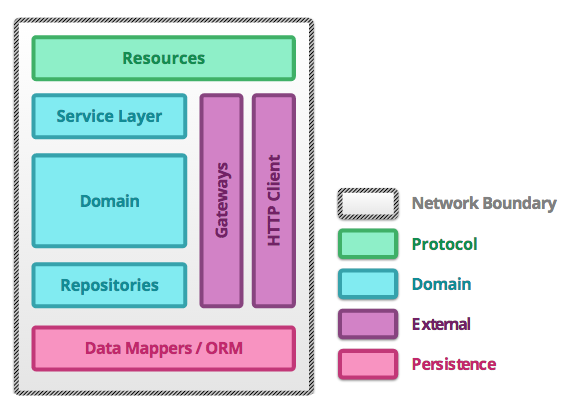
\includegraphics[width=6cm]{img/microservice_structure_example}
    \caption{Structuur van een architectuur met microservices (\cite{toby_clemson_testing_2014}) }
    \label{fig:microservice_structure_example}
\end{wrapfigure}


Een programma opsplitsen in componenten, met één verantwoordelijkheid, zorgt ervoor dat het meer schaalbaar is. Containers en unikernels helpen hierbij. Het opstarten van een nieuwe instantie van een microservice neemt minder tijd in beslag dan een nieuwe instantie dan een monoliet.

Bij microservices zal de topologie van het probleemdomein goed gekend moeten zijn. Starten met het gebruiken van microservices architecture wanneer men het domein niet goed kent, vraagt om problemen. Het ontwerpen van een microservices architectuur moet goed gebeuren. Anders kan later gelopen worden op problemen met de gehele architectuur en moeten andere microservices worden herschreven. Een monolithische architecture zal beter kunnen reageren op dit probleem. Als men later het domein kent kunnen we een microservices architecture gebruiken. Hiervoor moet de monoliet modulair geschreven worden. Modulariteit is een vanzelfsprekende bouwsteen binnen programmeren dus we kunnen hiervan uitgaan.

De complexiteit van een monoliet wordt overgebracht naar het communiceren en het behouden van de consistentie van de microservices. Verder wordt ook het opstellen de architectuur moeilijker. Dit betekent dat er meer werk komt te liggen bij systeembeheerders.

Het voordeel van een microservices architecuur is dat de microservices van elkaar gescheiden zijn. Het gebruik van een nieuwe technologie of framework is niet een groot probleem meer, omdat de microservices los van elkaar staan. Er kan dus een andere programmeertaal gebruikt worden zolang de communicatie tussen de microservices consistent blijft.

De communicatie van de microservices gebeurd via het netwerk. Dit maakt het mogelijk om microservices op verschillende virtuele machines of containers te laten werken. Het concept van software defined network (\cite{garcia_villalba_trends_2015}) neemt veel complexiteit weg van de communicatie.

\begin{wrapfigure}{r}{0.4\textwidth}
    \centering
    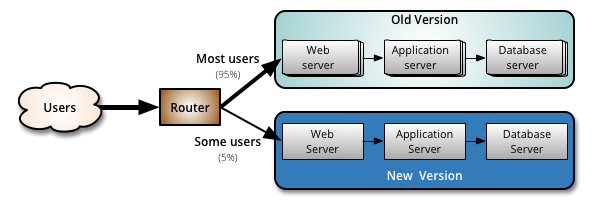
\includegraphics[width=6cm]{img/canary-release}
    \caption{Voorbeeld van een canary release (\cite{danilo_sato_canaryrelease_2014})}
    \label{fig:canary-release}
\end{wrapfigure}

Een monolithische architectuur opstellen in productie is relatief simpel tegenover een microservices architectuur. Wanneer er een nieuwe versie moet worden opgesteld in productie kan gebruik worden gemaakt van blue-green deployment (\cite{martin_fowler_bluegreendeployment_2016}). Waarbij we een oude en nieuwe versie hebben van de architectuur en de router het verkeer verlegd naar de nieuwe architectuur. Dit zorgt voor een gemakkelijk overgang.

Bij microservices kan gebruik gemaakt worden van een canary release strategie (\cite{danilo_sato_canaryrelease_2014}). Hier wordt weer een nieuwe versie opgesteld met de laatste veranderingen van de architectuur. De router gaat een deel van het verkeer naar de nieuwe architectuur versturen. Naarmate de tijd vordert, wordt het vertrouwen in de nieuwe versie nagegaan. Als het vertrouwen is toegenomen dan zal meer verkeer naar de nieuwe versie worden gestuurd. Zo kan men problemen nagaan en er sneller op reageren. Uiteindelijk krijgt de oude versie geen verkeer meer en wordt alleen de nieuwe versie gebruikt.

De systeembeheerder krijgt meer werk omdat er nu tientallen microservices moeten beheerd worden in plaats van één grote applicatie. Het beheren van deze microservices en hun logs wordt een belangrijke bron van informatie binnnen de architectuur. Men kan zeggen dat deze microservices simpeler zijn om te verstaan omdat de functionaliteit per microservices beperkt is. Sommige halen aan dat het de complexiteit die we niet meer tegenkomen in de applicatie nu terechtkomt bij het samen laten werken van de microservices.

De rol van systeembeheerder zal nauwer komen te liggen bij die van software ontwikkelaar. Er moet ook meer communicatie gebeuren tussen de systeembeheerders en software ontwikkelaars. De structuur van de architectuur moet samen besproken worden om een inzicht te krijgen in de uiteindelijke oplossing. Een microservices architectuur brengt deze twee groepen dichter bij elkaar. Meer informatie over de veranderingen die microservices hebben op systeembeheerders is te vinden in volgende thesis: \cite{balalaie_microservices_2016}.

\chapter{Immutable Infrastructure}

Unikernels vraagt ook een verschuiving van de manier waarop de infrastructuur en architectuur van een programma beheert wordt. Immutable infrastructure (\cite{martin_fowler_phoenixserver_2012}) is een opkomende gedachtegang. Er wordt geen enkele verandering aangebracht aan de programma's die zich in productie bevinden. Als er een probleem is dan wordt een nieuwe versie in productie geplaatst. Dit is al te zien bij sommige cloud providers die werken door middel van een git push om de voormalige versie te vervangen. Dit zorgt voor een hogere mate aan veiligheid en de hele cyclus van ontwikkelen naar productie wordt veel kleiner.

Canary releases zijn hierbij een ideale strategie voor veranderingen in de architectuur van het programma aan te brengen.

Een nieuw gegeven is ook dat infrastructuur meer wordt benaderd zoals programmeren (\cite{morris_infrastructure_2016}). Dit doen we door de infrastructure uitermate te testen en herhaalbare patronen te gebruiken. Ook wordt de configuratie bijgehouden in versie beheer. Door dit te doen krijgen we een beeld van wat er gebeurd met de infrastructuur door de tijd heen. Dit geeft de systeembeheerder de mogelijkheid om problemen terug te leiden naar één verandering. Het is belangrijk dat er steeds kleine veranderingen gebeuren zodat problemen gemakkelijker kunnen herleid worden naar één oorzaak. Gebruik maken van versie beheer zal niets uitmaken wanneer tientallen wijzigingen zijn gebundeld in één verandering.

\chapter{Conclusie}
\label{ch:conclusie}

Het efficiënt gebruiken van de middelen van de productieomgeving is een belangrijk gegeven, wanneer IT een groter deel uitmaakt van de meeste bedrijven. Innoveren om deze omgeving beter te gebruiken is broodnodig. Virtuele machines, containers en unikernels zijn maar enkele innovaties die dit doen. Deze bachelorproef richt zich vooral op de rol van systeembeheerder binnen bedrijven. Software containers hebben al gezorgd voor grotere veranderingen binnen de meeste bedrijven. Doorheen de bachelorproef werd gekeken naar nieuwe innovaties, vooral unikernels, die een invloed kunnen hebben op de rol van systeembeheerder.

De eerste onderzoeksvraag, waarop een antwoord kan worden gegeven, heeft betrekking tot de competenties van de systeembeheerder. Zoals al eerder is aangehaald is een architectuur van microservices van uiterst belang wanneer men unikernels wil gebruiken. De rol van systeembeheerder zal meer bestaan uit het communiceren met het software ontwikkelingsteam en de structuur van de architectuur uitwerken. Door microservices te gebruiken, wordt het opzetten van programma's een grotere taak. Het beheren en opstellen zal moeten gebeuren door de systeembeheerder en het software ontwikkelingsteam. De logs geven inzicht in de staat van de architectuur en het interpreteren van de logs zal met meer gemak gebeuren door het team dat het ontwikkeld heeft. Een nieuwe rol die gedeeltelijk bestaat uit software ontwikkelaar en systeembeheerder zal een betere werking als gevolg geven. Communicatie wordt ook van vitaal belang om ongename verassingen tegen te gaan.

De volgende onderzoeksvraag behandelt het opzetten van de architectuur. Doordat het programma bestaat uit meerdere microservices, moeten deze microservices met elkaar in verbinding staan voor een werkend programma te hebben. Software defined network en orchestratie frameworks kunnen hierbij helpen maar het wordt niet eenvoudiger om programma's op te stellen en te beheren. Microservices vermindert complexiteit in de broncode maar deze verhuist naar het opstellen en het onderhouden van programma's.

De use cases van containers en unikernels komen overeen met elkaar. Software containers zijn matuur en kunnen gerust gebruikt worden in productie. Unikernels heeft nog een lange weg te gaan om een mature status te bereiken. Het gebruiken van unikernels in productie bij algemen use cases is niet aan te raden. De voordelen van unikernels zijn duidelijk, maar er moet nog een duidelijker ecosysteem rond gevormd worden om een betere keuze te worden dan containers in sommige use cases. En compleet vervangen zal niet gebeuren, omdat er tegen veel moeilijkheden wordt gestoten bij het debuggen van unikernels. Dit is een belangrijke kwestie die nog moet behandelt worden.

Unikernels vragen ook een grote verandering van architectuur wanneer er nog geen gebruik wordt gemaakt van microservices. Alle twee deze technologiën tegelijk introduceren kan leiden tot een moeizame overgang met slechte ervaringen.

De beveiliging dat bereikt wordt bij unikernels is niet te onderschatten, maar er moet veel worden opgeofferd om dit te gebruiken in een zinvolle situatie. Er zijn alle niche use cases waar unikernels kunnen gebruikt worden zoals middleboxes, maar het domein waarin deze gebruikt worden is beperkt.

De uiteindelijke conclusie is dat unikernels veel goeds belooft en tevens waarmaakt. Er zijn wel opofferingen die moeten gebeuren die een gevolg hebben op de hele architectuur en infrastructuur. Als er een ecossysteem rond unikernels wordt gevormd zoals bij containers (Docker), dan zullen unikernels gebruikt kunnen worden in een algemenere context.

\bibliographystyle{apa}
\bibliography{tin-bachproef}

%%---------- Back matter -------------------------------------------------

\listoffigures
\listoftables

\end{document}
